\begin{center}
\textbf{\Large Точки пересечения биссектрис}\\
\textit{19.07.16}
\end{center}

\epigraph{\it две параллельные прямые\\
живут в евклидовом мирке\\
и бегают пересекаться\\
в мир лобачевского тайком}{Пирожок}

\begin{problems}
\item В треугольнике $ABC$ $\angle A=\alpha$. Найдите угол между биссектрисами $BB_1$ и $CC_1$.

\item Может ли точка пересечения биссектрис лежать на средней линии треугольника?

\begin{center}
	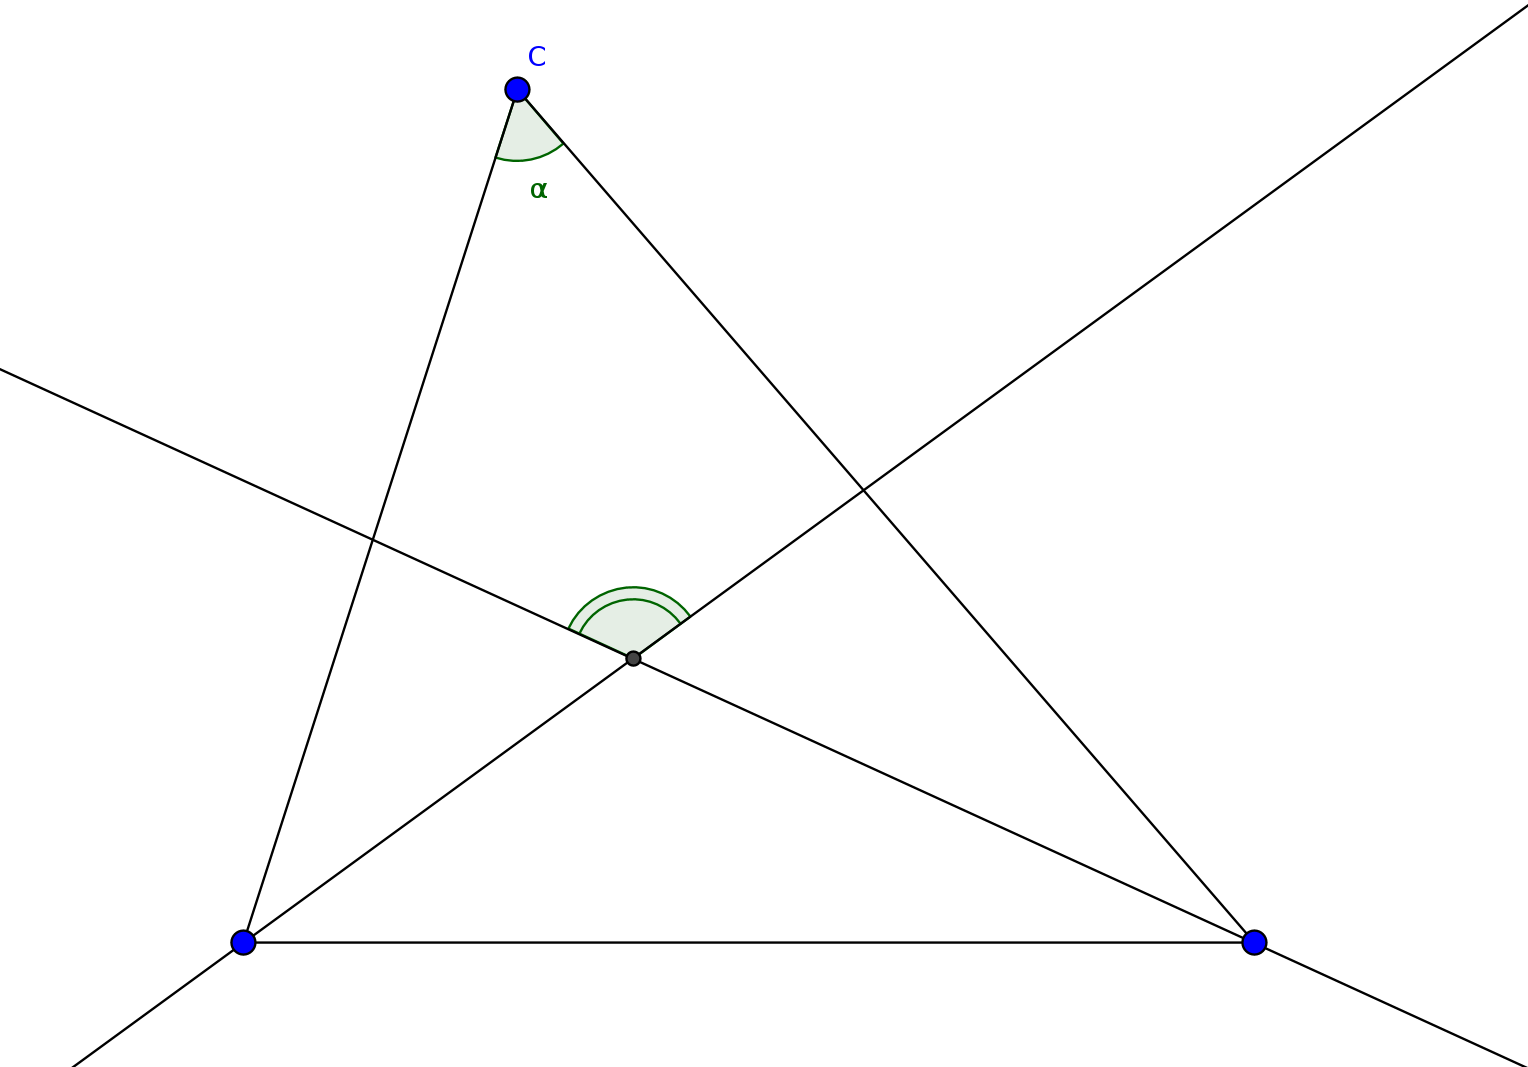
\includegraphics[width=.45\textwidth]{incen01}
	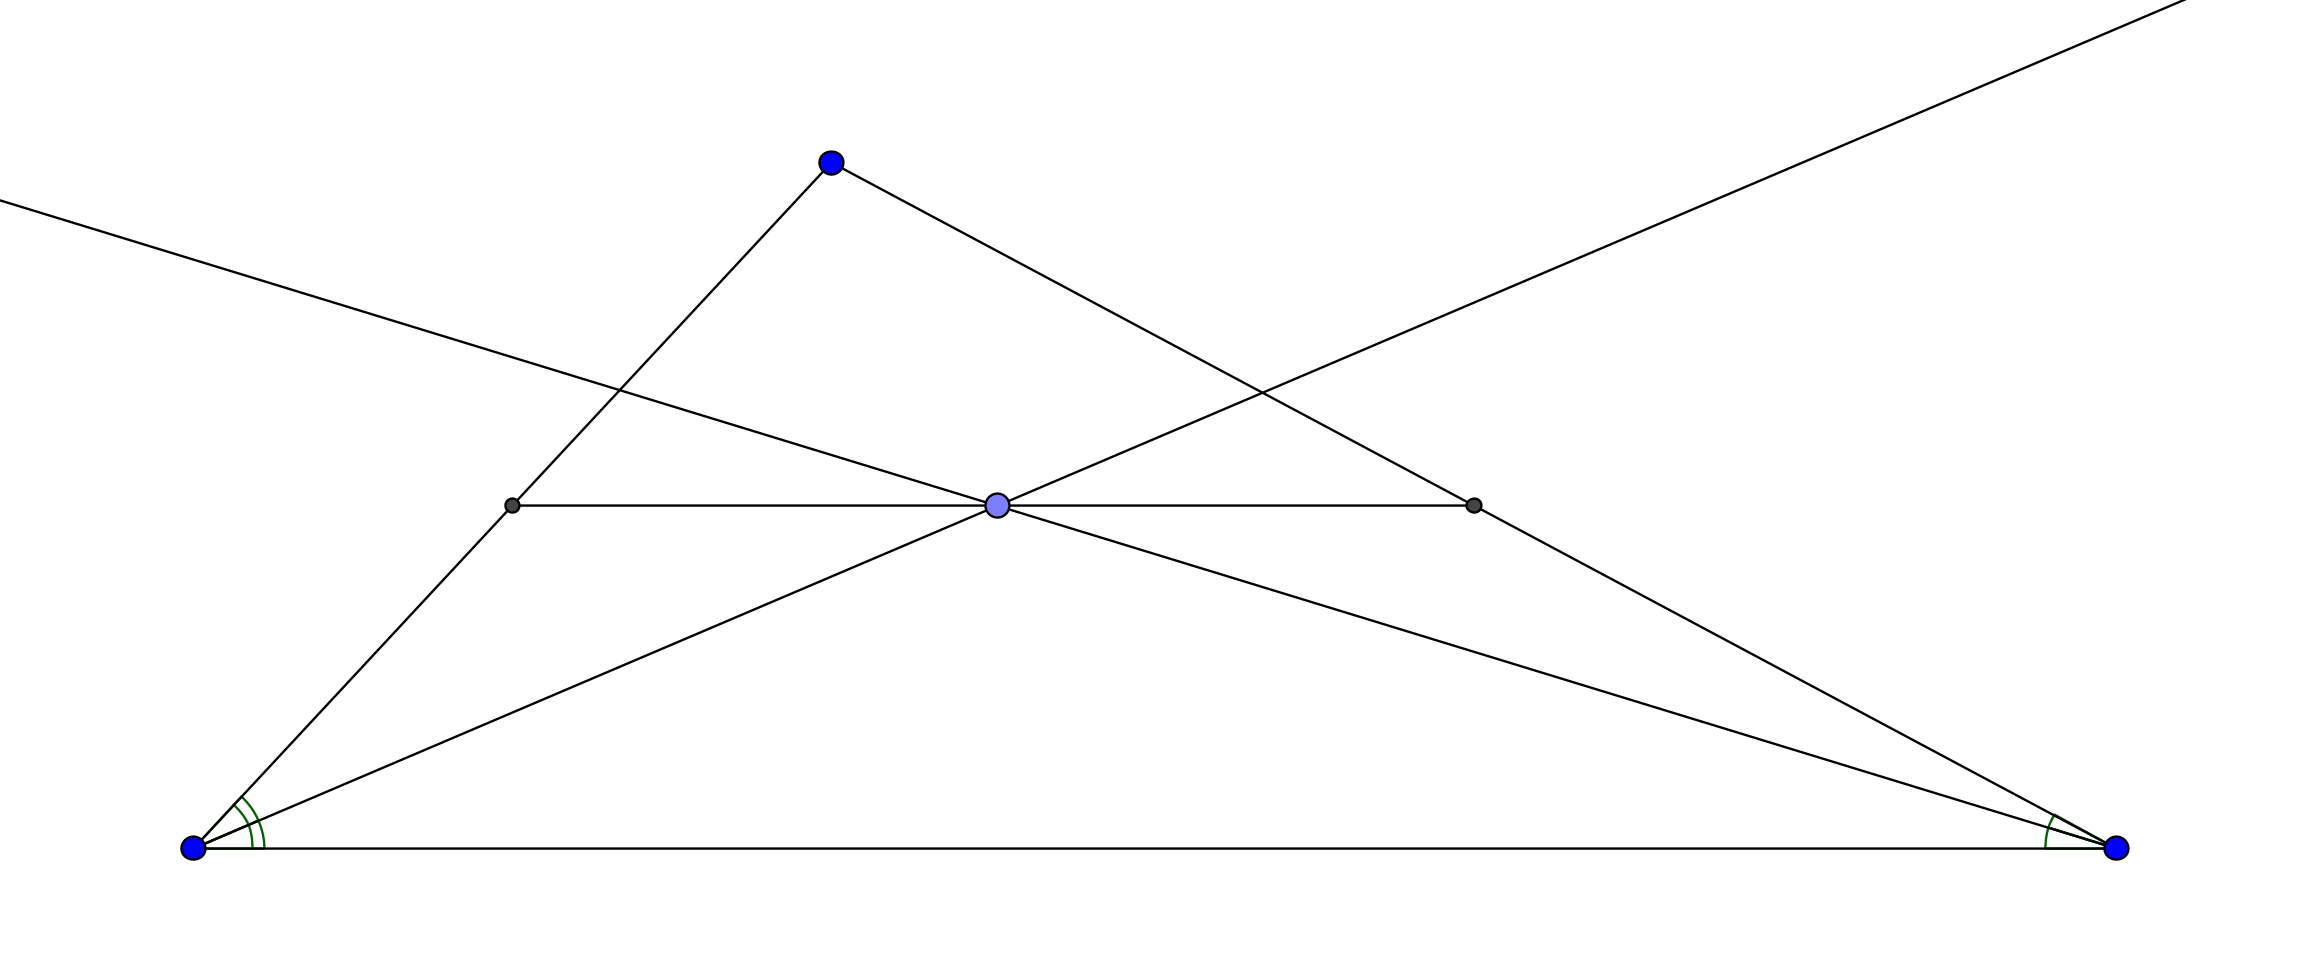
\includegraphics[width=.45\textwidth]{incen02}
\end{center}

\item В четырёхугольнике $ABCD$ $\angle B=\angle C=146^{\circ}$. Биссектриса угла $D$ пересекает серединный перпендикуляр к стороне $BC$ в точке $O$. Найдите $\angle AOD$.

\item В выпуклом шестиугольнике $ABCDEF$, все углы которого тупые, $\angle A=\angle B$, $\angle C=\angle D$, $\angle E=\angle F$. Докажите, что серединные перпендикуляры к его сторонам $AB, CD, EF$ пересекаются в одной точке.

\item Биссектрисы двух соседних углов четырехугольника пересекаются в середине его стороны. Докажите, что либо у этого четырехугольника равны два угла, либо две стороны параллельны. 

\item От угла равностороннего треугольника со стороной $1$ отрезали меньший треугольник так, что биссектриса его внешнего угла делит пополам сторону исходного треугольника, противоположную данному углу. Найдите периметр отрезанного треугольника.

\item Дан четырёхугольник $ABCD$, в котором $\angle ABD=\angle DBC=60^{\circ}$, $\angle ADB=40^{\circ}$, а $\angle BDC=70^{\circ}$. Найдите угол между его диагоналями.

\begin{center}
	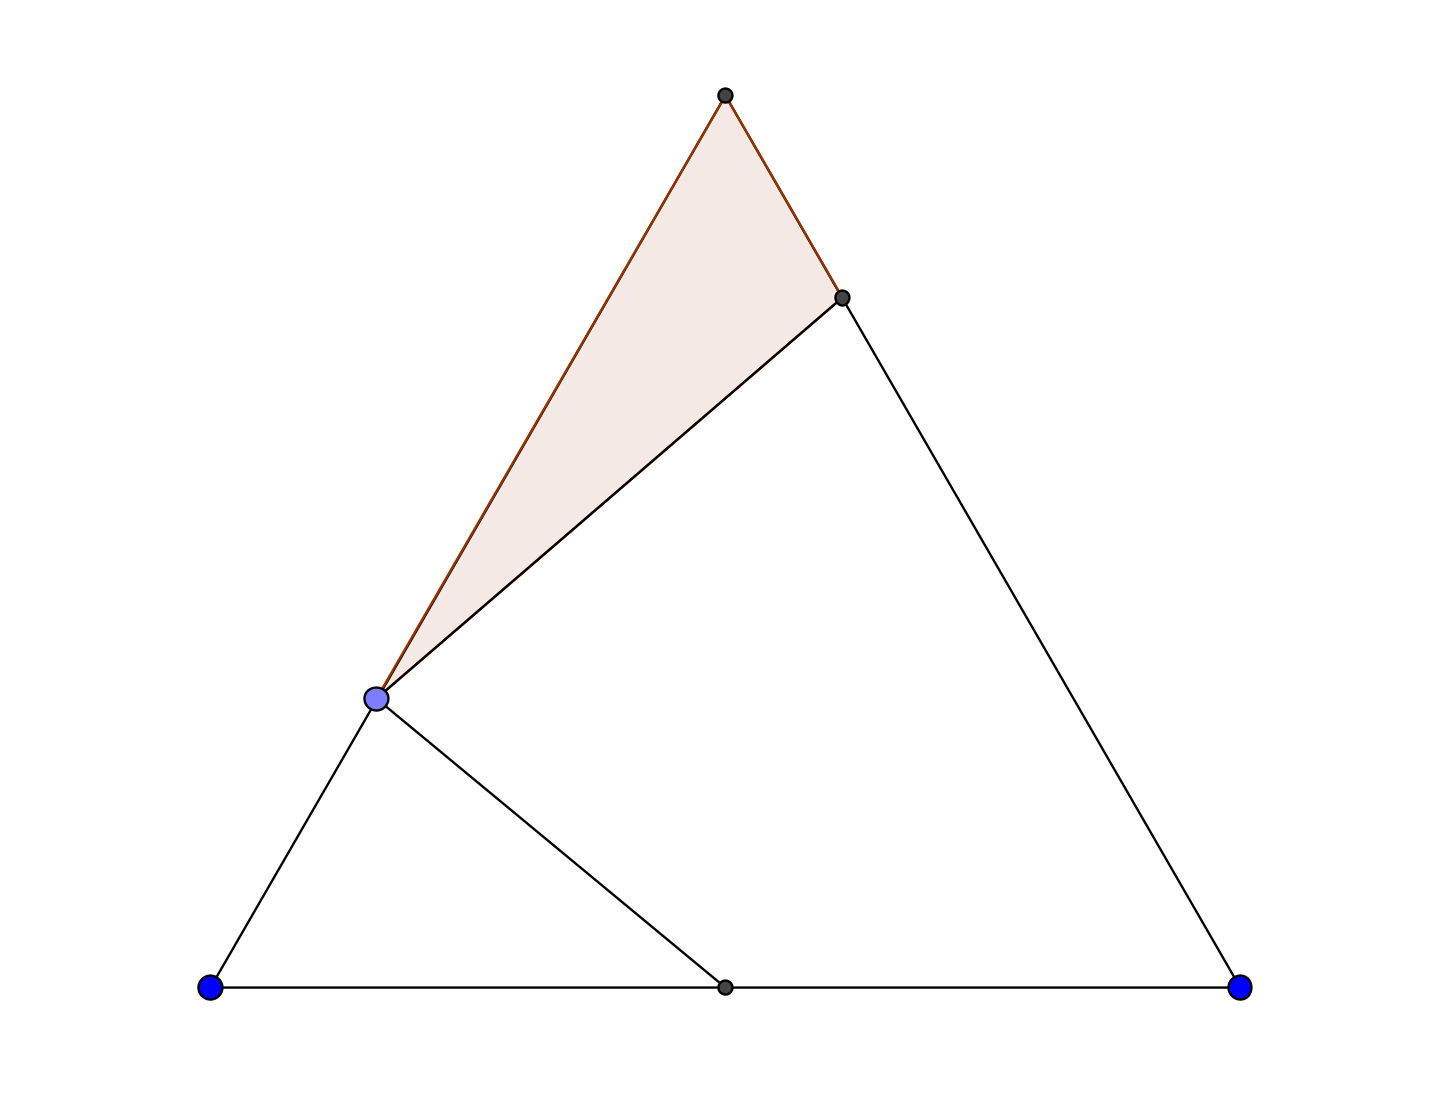
\includegraphics[width=.45\textwidth]{incen03}
	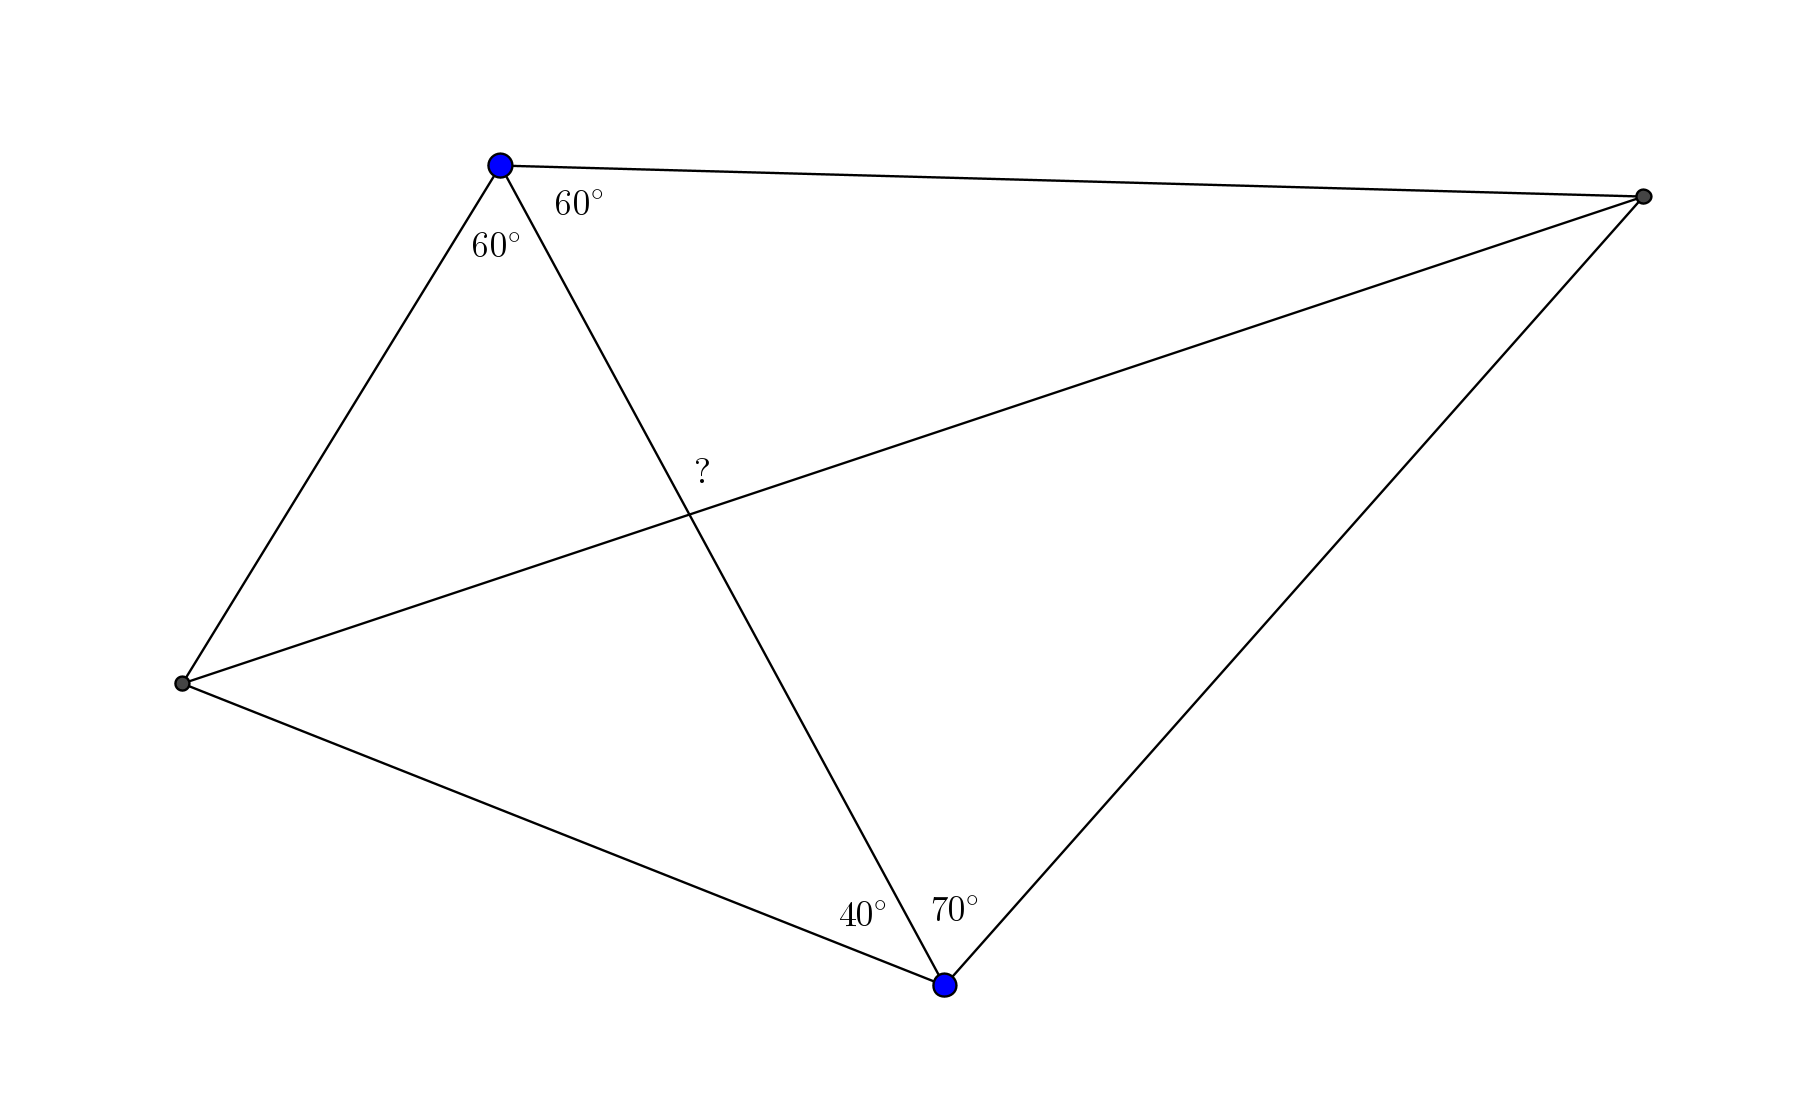
\includegraphics[width=.45\textwidth]{incen04}
\end{center}

\item В треугольнике $ABC$ угол $A$ равен $60^{\circ}$. На сторонах $AB$ и $AC$ выбраны точки $K$ и $L$ соответственно так, что $BK = KL = LC$. Докажите, что угол $KLC$ в два раза больше угла $ABC$.
%центр вневписанной окружности

%\item На~сторонах $AB$ и~$AD$ единичного квадрата $ABCD$ выбраны точки $N$ и~$P$ соответственно. Причем периметр треугольника $ANP$ равен 2. Докажите, что $\angle NCP=45^{\circ}$.

\end{problems}